\documentclass[a4paper,12pt]{jarticle}
\usepackage[dvipdfmx]{graphicx}
\usepackage{amsmath}
\usepackage{subfigure}
\usepackage{comment}
\usepackage{listings}

\setlength{\hoffset}{0cm}
\setlength{\oddsidemargin}{-3mm}
\setlength{\evensidemargin}{-3cm}
\setlength{\marginparsep}{0cm}
\setlength{\marginparwidth}{0cm}
\setlength{\textheight}{24.7cm}
\setlength{\textwidth}{17cm}
\setlength{\topmargin}{-45pt}

\renewcommand{\baselinestretch}{1.6}
\renewcommand{\floatpagefraction}{1}
\renewcommand{\topfraction}{1}
\renewcommand{\bottomfraction}{1}
\renewcommand{\textfraction}{0}
\renewcommand{\labelenumi}{(\arabic{enumi})}
%\renewcommand{\figurename}{Fig.} %図をFig.にする


%図のキャプションからコロン:を消す
\makeatletter
\long\def\@makecaption#1#2{% #1=図表番号、#2=キャプション本文
\sbox\@tempboxa{#1. #2}
\ifdim \wd\@tempboxa >\hsize
#1 #2\par 
\else
\hb@xt@\hsize{\hfil\box\@tempboxa\hfil}
\fi}
\makeatother
% 

\title{車両制御特論 \\
レポート1\\
}
\author{\vspace{40mm}\\
九州工業大学大学院 \hspace{0mm} 工学府\\
機械知能工学専攻\ \hspace{0mm} 知能制御工学コース \\
\vspace{5mm}\\
所属:\ 西田研究室\\
学籍番号:\ 16344217\\
提出者氏名:\ 津上 \hspace{0mm} 祐典\\\vspace{5mm}\\ }
\date{平成28年\ 7月\ 19日}

\begin{document}

%表紙
\titlepage
\maketitle
\thispagestyle{empty}

\newpage
%%%%%%%%%%%%%%%%%%%%%%%%%%%%
\section{与えられたシステム}
%%%%%%%%%%%%%%%%%%%%%%%%%%%
学籍番号より決定した解析するシステムは
\begin{eqnarray}\label{equ:sys}
 \begin{cases}
  \dot{x}(t) = -4x(t) + 6u_{4}(t)  \\
  u_{4}(t) = -2-\sin t &
 \end{cases}
\end{eqnarray}
である.
%
%%%%%%%%%%%%%%%%%%%%%%%%%%%
\section{システムの解析解}
%%%%%%%%%%%%%%%%%%%%%%%%%%%
(\ref{equ:sys})式で示したシステムの解析解$x(t)$を導出する.
(\ref{equ:sys})式より
%
\begin{eqnarray}
 \dot{x}(t) &=& -4x(t) + 6(-2-\sin t) \\
 \dot{x}(t) &=& -4x(t) -12 -6\sin t
\end{eqnarray}
%
となる.上式の両辺をラプラス変換し,整理すると,
%
\begin{eqnarray}
 sX(s) + 5 & = & -4X(s) - \frac{12}{s} - \frac{6}{s^2 + 1} \\
 (s+5)X(s) & = & -5 - \frac{12}{s} - \frac{6}{s^2 + 1} \\
 X(s) & = & -\frac{5}{s+4} - \frac{12}{s(s+4)} - \frac{6}{(s^2 + 1)(s+4)} \\
 X(s) & = & -\frac{5}{s+4} - 12 (\frac{\frac{1}{4}}{s} -
  \frac{\frac{1}{4}}{s+4}) -6(\frac{-\frac{1}{17}s+\frac{4}{17}}{s^2 +
  1}+\frac{\frac{1}{17}}{s+4}) \\
 X(s) & = & -\frac{40}{17}\frac{1}{s+4} + \frac{6}{17}\frac{s}{s^2 + 1}
  -\frac{24}{17}\frac{1}{s^2 + 1} -\frac{3}{s}
 \end{eqnarray}
となる.ただし,$X(s)$は$x(t)$をラプラス変換したものである.そして,上式
の両辺を逆ラプラス変換すればシステムの解析解
%
\begin{equation}
 x(t)  =  -\frac{40}{17}e^{-4t} + \frac{6}{17}\cos t -\frac{24}{17}\sin t -3
\end{equation}
%
を得る.
%%%%%%%%%%%%%%%%%%%%%%%%%%%%%%%%%%%%%%%%%%
\section{Simulink,MATLABのプログラム}
%%%%%%%%%%%%%%%%%%%%%%%%%%%%%%%%%%%%%%%%%%
(\ref{equ:sys})式で示されるシステムをSimulinkのモデルを図\ref{fig:model}に,MATLABのプログラ
ムをListing 1.に示す.
%
\begin{figure}[hbp]
 \begin{center}
  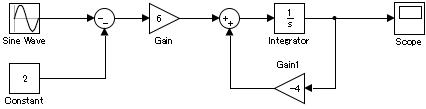
\includegraphics[scale=.7,bb = 0 0 426 109]{fig/model.jpg}
 \end{center}
 \caption{作成したsimulinkモデル}
 \label{fig:model}
\end{figure}
%
\begin{lstlisting}[basicstyle=\ttfamily\footnotesize,frame=single,caption=作成したMATLABのプログラム]
clc;
clear; 
clf; 

t=[0:0.1:100];
y = -(40/17)*exp(-4*t)+(6/17)*cos(t)-(24/17)*sin(t)-3;

axis([0 50 -10 100]),grid 
xlabel('t');  
ylabel('y');
plot(t,y)   
\end{lstlisting}


%%%%%%%%%%%%%%%%%%%%%%%%%
\section{得られた応答}
%%%%%%%%%%%%%%%%%%%%%%%%
%
得られた応答波形を図\ref{fig:text2}に示す.
\begin{figure}[hbp]
 \begin{center}
  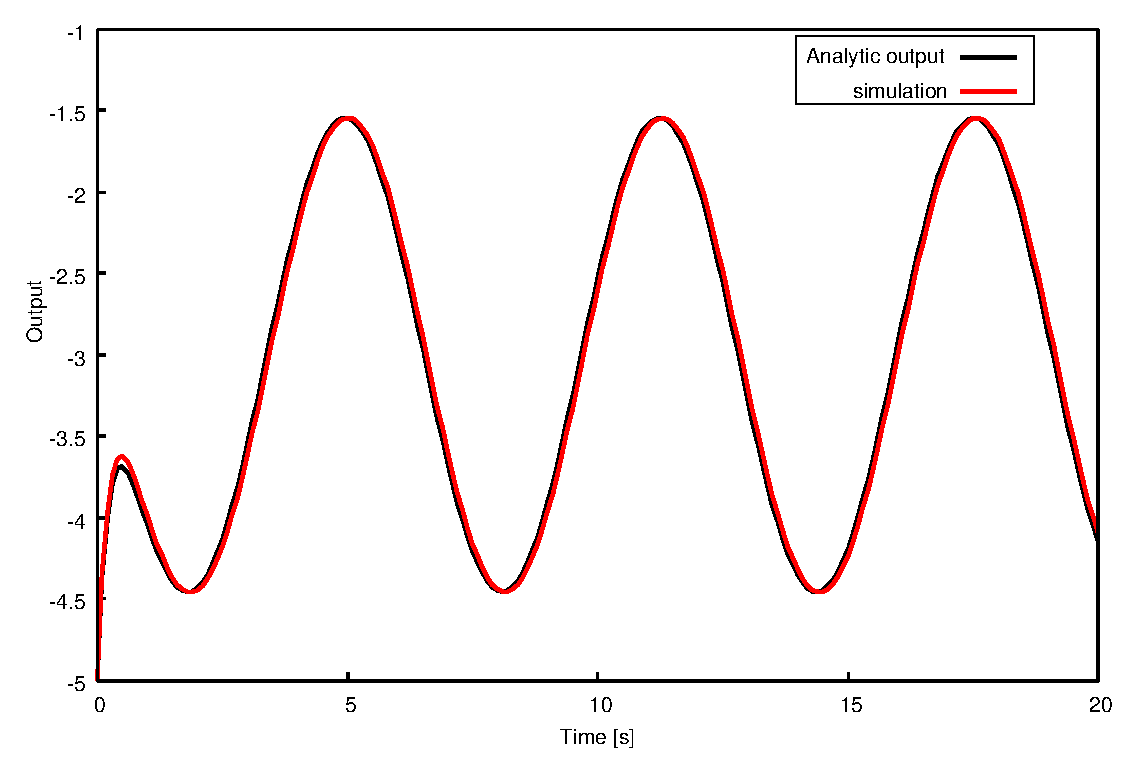
\includegraphics[width = 150 mm]{fig/text2.eps}
 \end{center}
 \caption{MATLABによるシミュレーション結果と解析解のプロットとの比較}
 \label{fig:text2}
\end{figure}
%
%%%%%%%%%%%%%%%%%%%%%%%%
\section{考察}
%%%%%%%%%%%%%%%%%%%%%%%%
特になし.
\end{document}
